\documentclass[crop,tikz]{standalone}

\usepackage{amsmath}
\usepackage{pgfplots}
\tikzset{>=latex}

\pgfplotsset{
  inverted/.style = {
    every axis legend/.append style={
      draw=white,
      fill=hardblack,
      text=white
    }
  },
  compat=1.16,
  every non boxed x axis/.append style={
    axis line style={-latex}
  },
  every non boxed y axis/.append style={
    axis line style={-latex}
  }
}

\begin{document}
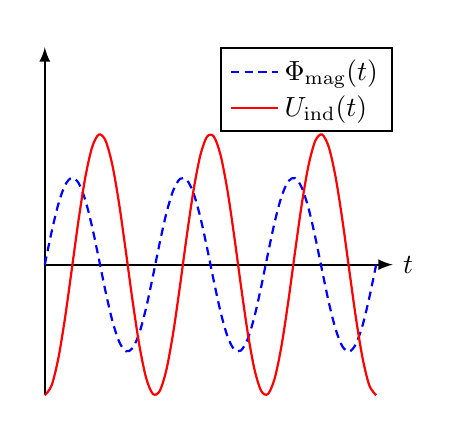
\begin{tikzpicture}
\begin{axis}[
  thick,
  width=6cm,
  height=6cm,
  domain={0}:{4*pi},
  samples=50,
  axis y line=middle,
  axis x line=middle,
  xlabel={$t$},
  ylabel={$\hphantom{x}$},
  xlabel style={right},
  ylabel style={above},
  xmin=0, xmax={4.2*pi},
  ymin=-1.5, ymax=2.5,
  xtick={\empty},
  xticklabels={\empty},
  ytick={\empty},
  yticklabels={\empty},
  legend cell align={left},
  legend style={at={(1,1)},anchor=north east},
  clip=false
  ]
  \addplot[blue,smooth,densely dashed] { sin(1.5*deg(x)) };
  \addlegendentry{$\Phi_{\text{mag}}(t)$};
  \addplot[red,smooth] { -1.5*cos(1.5*deg(x)) };
  \addlegendentry{$U_{\text{ind}}(t)$};
\end{axis}
\end{tikzpicture}
\end{document}
